\documentclass[12pt,a4paper,titlepage,headinclude,bibtotoc]{scrartcl}

%---- Allgemeine Layout Einstellungen ------------------------------------------

% Für Kopf und Fußzeilen, siehe auch KOMA-Skript Doku
\usepackage[komastyle]{scrpage2}
\pagestyle{plain}
\setheadsepline{0.5pt}[\color{black}]
\automark[section]{chapter}


%Einstellungen für Figuren- und Tabellenbeschriftungen
\setkomafont{captionlabel}{\sffamily\bfseries}
\setcapindent{0em}


%---- Weitere Pakete -----------------------------------------------------------
% Die Pakete sind alle in der TeX Live Distribution enthalten. Wichtige Adressen
% www.ctan.org, www.dante.de

% Sprachunterstützung
\usepackage[ngerman]{babel}

% Benutzung von Umlauten direkt im Text
% entweder "latin1" oder "utf8"
\usepackage[utf8]{inputenc}

% Pakete mit Mathesymbolen und zur Beseitigung von Schwächen der Mathe-Umgebung
\usepackage{latexsym,exscale,stmaryrd,amssymb,amsmath}


\usepackage[nointegrals]{wasysym}
\usepackage{eurosym}

% Anderes Literaturverzeichnisformat
%\usepackage[square,sort&compress]{natbib}
\usepackage{hyperref}
% Für Farbe
\usepackage{color}
\usepackage{graphicx}
\usepackage{wrapfig}
\usepackage{subfigure}

% Caption neben Abbildung
\usepackage{sidecap}

% Befehl für "Entspricht"-Zeichen
\newcommand{\corresponds}{\ensuremath{\mathrel{\widehat{=}}}}
% Befehl für Errorfunction
\newcommand{\erf}[1]{\text{ erf}\ensuremath{\left( #1 \right)}}

%Fußnoten zwingend auf diese Seite setzen
\interfootnotelinepenalty=1000

%Für chemische Formeln (von www.dante.de)
%% Anpassung an LaTeX(2e) von Bernd Raichle
\makeatletter
\DeclareRobustCommand{\chemical}[1]{%
  {\(\m@th
   \edef\resetfontdimens{\noexpand\)%
       \fontdimen16\textfont2=\the\fontdimen16\textfont2
       \fontdimen17\textfont2=\the\fontdimen17\textfont2\relax}%
   \fontdimen16\textfont2=2.7pt \fontdimen17\textfont2=2.7pt
   \mathrm{#1}%
   \resetfontdimens}}
\makeatother

%Honecker-Kasten mit $$\shadowbox{$xxxx$}$$
\usepackage{fancybox}

%SI-Package
\usepackage{siunitx}

%keine Einrückung, wenn Latex doppelte Leerzeile
\parindent0pt

%Bibliography \bibliography{literatur} und \cite{gerthsen}
%\usepackage{cite}
\usepackage{babelbib}
\selectbiblanguage{ngerman}

\begin{document}

\begin{titlepage}
\centering
\textsc{\Large Praktikum zur Einführung in die physikalische Chemie,\\[1.5ex] Universität Göttingen}

\vspace*{1cm}

\rule{\textwidth}{1pt}\\[0.5cm]
{\huge \bfseries
  V6: Dissoziationskonstante\\[1.5ex]
  einer schwachen Säure}\\[0.5cm]
\rule{\textwidth}{1pt}

\vspace*{3cm}


\begin{Large}
\begin{tabular}{ll}
Durchführende: &  Alea Tokita, Julia Stachowiak\\
Assistentin: & Annemarie Kehl\\
 Versuchsdatum: & 18.01.2016\\
 Datum der Abgabe: & 25.01.2016\\
\end{tabular}
\end{Large}

\vspace*{1cm}

\begin{Large}
\fbox{
  \begin{minipage}[t][5cm][t]{5cm} 
  \textbf{Werte:}\\
  \end{minipage}
}
\end{Large}

\end{titlepage}

\tableofcontents

\newpage

\section{Theoretische Grundlagen}

Die Dissoziationskonstante der schwachen Säure p-Nitrophenol soll mittels Photometrie gemessen werden. \\
Säuren bilden in wässriger Lösung folgendes Gleichgewicht; $\mathrm{A^-}$ beschreibt den Säurerest.\\

\begin{equation}
\mathrm{HA}  \rightleftharpoons \mathrm{H^+} + \mathrm{A^-}
\end{equation}

Die Lage des Gleichgewichtes ist durch das Massenwirkungsgesetz definiert:\\

\begin{equation}
K_\mathrm{c} =\frac{c(\mathrm{H+}*c{A^-}{c(HA)}
\end{equation}

Der $\mathrm{pK_s}$-Wert ist der negativ dekadische Logarithmus von $\mathrm{K_S}$; der PH-Wert der negativ dekadische Logarithmus der Oxoniumionenkonzentration:






In Lösung bildet p-Nitrophenol folgendes Gleichgewicht:

\centering
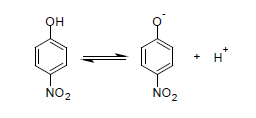
\includegraphics[scale=1]{Strukturformel}

Die dissoziierte und undissoziierte Form weisen eine unterschiedliche Lichtdurchlässigkeit auf.



\section{Bestimmung der Dissoziationskonstante}




\subsection{Versuchsaufbau}
+ Versuchsaufbau; Photometer

\subsection{Durchführung}




\section{Auswertung}
Im Versuch wird die Messung der Extinktion für jeden pH, sowie für $E_{\infty}$, sechsmal durchgeführt. Anschließend wird daraus für jeden pH der Mittelwert der Extinktion gebildet. Es ergeben sich folgende Mittelwerte:

\begin{table} [h]
\begin{tabular} {| p {1,5 cm}|| p {3 cm}|}
  \hline\\
  pH & $\overline{E}$\\\hline
  $6,2$& $0,18$\\\hline
  $6,4$& $0,255$\\\hline
  $6,6$& $0,347$\\\hline
  $6,8$& $0,463$\\\hline
  $7,0$& $0,659$\\\hline
  $7,2$& $0,827$\\\hline
  $7,4$& $0,948$\\\hline
  $7,6$& $1,044$\\\hline
 

\end{tabular}
\end{table}
Für   
\end{document}
